\section{Transport of relation lattices}\label{sec:lattice}
Throughout this section $p_1<\dots<p_k$ are primes coprime to the moduli $b,b'$ and $\Lambda_b=\ker\chi_b$.

\subsection{Lattice order from group orders}
\begin{proposition}\label{prop:E22}
$[\Z^k:\Lambda_b]=|H_b|$; $\Lambda_b\cap\Lambda_{b'}=\Lambda_{\mathrm{lcm}(b,b')}$; hence $\Lambda_b\subseteq\Lambda_{b'}\iff|H_{\mathrm{lcm}(b,b')}|=|H_b|$.
\end{proposition}
\prov{CW-0457}{E2-2}{PROVED}{FULL}
\begin{proof}
$\chi_b:\Z^k\to H_b$ is onto with kernel $\Lambda_b$, giving the index. By the Chinese remainder theorem $\chi_b(\alpha)=1=\chi_{b'}(\alpha)$ iff $\chi_{\mathrm{lcm}}(\alpha)=1$. If $\Lambda_b\subseteq\Lambda_{b'}$ then $\Lambda_{\mathrm{lcm}}=\Lambda_b$, so the indices agree. Conversely $\Lambda_{\mathrm{lcm}}\subseteq\Lambda_b$ with equal finite index gives equality, so $\Lambda_b=\Lambda_{\mathrm{lcm}}\subseteq\Lambda_{b'}$. \qedhere
\end{proof}

\subsection{A decision criterion}
\begin{theorem}[lattice transport]\label{thm:P2T1}
Let $m_i=\ord_b(p_i)$. The following are equivalent: (a) $\Lambda_b\subseteq\Lambda_{b'}$; (b) $p_i\bmod b\mapsto p_i\bmod b'$ extends to a well-defined homomorphism $H_b\to H_{b'}$; (c) every element of the finite set $\{m_ie_i\}\cup\{\alpha\in\prod[0,m_i):\chi_b(\alpha)=1\}$ lies in $\Lambda_{b'}$.
\end{theorem}
\prov{CW-0467}{P2-T1}{PROVED}{FULL}
\begin{proof}
A homomorphism $\varphi$ with $\varphi\circ\chi_b=\chi_{b'}$ exists iff $\ker\chi_b\subseteq\ker\chi_{b'}$ (universal property of the surjection $\chi_b:\Z^k\to H_b$); this is (a)$\iff$(b). For (c): $m_ie_i\in\Lambda_b$. Any $\alpha\in\Z^k$ is $\sum_it_im_ie_i+r$ with $r\in\prod[0,m_i)$, and $\alpha\in\Lambda_b$ iff $r\in\Lambda_b$; so the displayed set generates $\Lambda_b$, and $\Lambda_{b'}$ is a group. \qedhere
\end{proof}
\begin{corollary}[denominators]\label{cor:denominators}
If $b'\mid b$ then $\Lambda_b\subseteq\Lambda_{b'}$. This is sufficient, not necessary, and does not give strict inclusion.
\end{corollary}
\prov{CW-0467}{P2-T1}{PROVED}{FULL}
\begin{proof}
A congruence modulo $b$ implies the same congruence modulo $b'$. For non-necessity take $b=5$, $b'=4$, primes $3,7$: $\Lambda_5=\{a\equiv b\ (4)\}$ and $\Lambda_4=\{a\equiv b\ (2)\}$ (see the proof of \cref{thm:P2TF1}), so $\Lambda_5\subsetneq\Lambda_4$ though $4\nmid5$ and $5\nmid4$. Equality can occur: for the primes $\{5,17,29\}$ one has $5,17,29\equiv-1\pmod 3$ and $\equiv5\pmod{12}$ with $5^2\equiv1$, so $\Lambda_3=\Lambda_{12}=\{\alpha:\sum\alpha_i\text{ even}\}$ although $b=3\neq12=b'$. \qedhere
\end{proof}
This correction (ER-16) replaces the earlier phrase ``denominator divisibility is neither necessary nor sufficient'' of the first release; the sufficiency statement is the form used here.

\begin{lemma}[order rule]\label{lem:orderrule}
Let $n_i=\ord_{b'}(p_i)$. If $g\in\Z^k$ has $|g_i|\ge n_i$ for some $i$ and $g\ne\pm n_ie_i$, then $g\notin\Gr(\Lambda_{b'})$.
\end{lemma}
\prov{CW-0468}{P2-L2}{PROVED}{FULL}
\begin{proof}
$h=\mathrm{sign}(g_i)\,n_ie_i\in\Lambda_{b'}$ is nonzero, $h\cm g$ and $h\ne g$. \qedhere
\end{proof}
This is an $O(k)$ \emph{necessary} condition for a vector to survive as a target Graver move; it is not sufficient.

\subsection{Fibre inclusion versus lattice inclusion}
\begin{proposition}\label{prop:fibre-vs-lattice}
(a) If $\Lambda\subseteq\Lambda'$ and the box is common, then $F(\Lambda,Q)\subseteq F(\Lambda',Q)$. (b) The converse is false: $x=484/3$ and $x'=484/7$, primes $(2,11)$, box $[0,1]^2$, have $F=F'=\{(1,1)\}$, yet $\Lambda_3=\{a+b\text{ even}\}$ and $\Lambda_7=\{a\equiv b\ (3)\}$ are incomparable. (c) If $F\subseteq F'$ and $\mathrm{span}_\Z F=\Lambda$, then $\Lambda\subseteq\Lambda'$.
\end{proposition}
\prov{CW-0459}{E2-4}{PROVED}{ADAPTED}
\begin{figure}[tbp]\centering
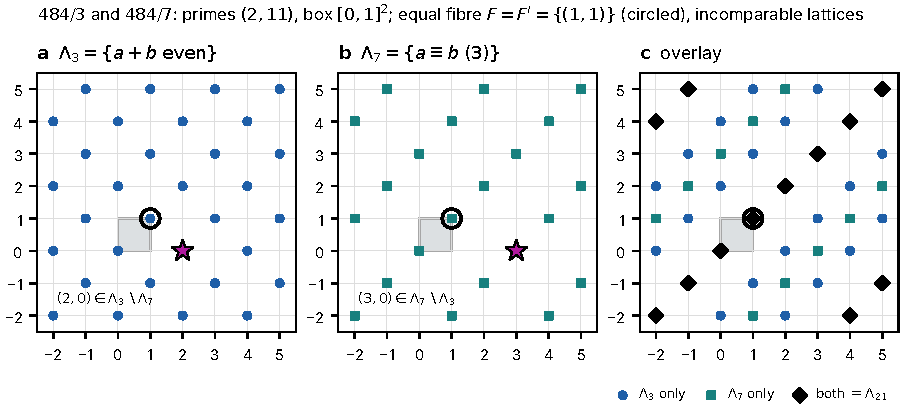
\includegraphics[width=0.98\textwidth]{fig02_equal_fibres}
\caption{Equal fibres, incomparable lattices (\cref{prop:fibre-vs-lattice}(b); \emph{exact computation}): $x=484/3$ and $x'=484/7$, primes $(2,11)$, box $[0,1]^2$, window $[-2,5]^2$ of the infinite lattices. (a)~$\Lambda_3=\{a+b\ \text{even}\}$; (b)~$\Lambda_7=\{a\equiv b\ (3)\}$; (c)~overlay, with $\Lambda_3\cap\Lambda_7=\Lambda_{21}$. The shaded unit square is the box and the point $(1,1)$ is the common fibre $F=F'$. The stars are the exact witnesses $(2,0)\in\Lambda_3\setminus\Lambda_7$ and $(3,0)\in\Lambda_7\setminus\Lambda_3$: the lattices are incomparable although the fibres coincide, so the spanning hypothesis in \cref{prop:fibre-vs-lattice}(c) cannot be dropped.}\label{fig:equalfibres}
\end{figure}
\begin{proof}
(a) is immediate. (c): $F\subseteq F'\subseteq\Lambda'$; take the span. (b): $484=2^2\cdot11^2$, so $d^2\mid484$ iff $d\mid22$; $22\equiv1$ modulo $3$ and $7$, while $2,11\not\equiv1$; thus $D=D'=\{22\}$, $F=F'=\{(1,1)\}$ for the box $[0,1]^2$. Modulo $3$: $2\equiv11\equiv-1$, so $\chi_3(a,b)=(-1)^{a+b}$. Modulo $7$: $2$ has order $3$ and $11\equiv2^2$, so $\chi_7(a,b)=2^{a+2b}$, trivial iff $a\equiv b\pmod 3$. Then $(2,0)\in\Lambda_3\setminus\Lambda_7$ and $(3,0)\in\Lambda_7\setminus\Lambda_3$. \qedhere
\end{proof}
The adapted statement (c) is the content of Lemma E2-4 (``no shrinking''): along a collective step with $D(x)\subseteq D(\Cmap(x))$ (Foundations Vol.~II, Thm.~1.3, F.T31~\cite{FoundII}; cited, not reproved) one has $F\subseteq F'$, so a spanning fibre forces $\Lambda\subseteq\Lambda'$. Also, every denominator along an orbit divides $G(x_0)$ (E2-3, resting on the same inherited facts), so the lattices along an orbit all contain $\Lambda_{G(x_0)}$ in fixed coordinates. The spanning hypothesis must accompany every use of (c) (ER-14).
\prov{CW-0458}{E2-3}{PROVED}{ADAPTED}

\subsection{Corpus statistics (finite-exact)}
\begin{proposition}[FINITE-EXACT; source scope]\label{prop:corpus}
In the exact corpus of $596$ admissible non-EQUAL transitions of the source ($582$ with $k=2$, $14$ with $k=3$) one finds ENLARGE $275$, SHRINK $262$, INCOMPARABLE $59$; in every row $F\subseteq F'$. No SHRINK or INCOMPARABLE row has a spanning source fibre ($321/321$). If $b\mid b'$ the class is SHRINK in all $199$ such rows; if $b'\mid b$ it is ENLARGE in all $154$.
\end{proposition}
\prov{CW-0472}{P2-D}{FINITE-EXACT}{FINITE}
These numbers are a computation in the stated corpus, reported from the release; the planar sampling windows of the first release were incomplete for boxes with $q_1<q_2$, and all $326$ geometry verdicts were recomputed with full-box certificates in the next release with $0$ verdicts changed (ER-18); they are not re-derived here and are not extrapolated. Their consequence for this manuscript is only qualitative: transitions with SHRINK or INCOMPARABLE lattices occur under $\Cmap$ (so ``the lattice never shrinks'' is not a law, ER-14), and transport theorems must either assume $\Lambda\subseteq\Lambda'$ or avoid lattice comparison.
